%!TEX root = ../proceedings.tex
% \subsection{Assigning Work}
\textit{Who gets new work opportunities first is a contentious issue which should be negotiated by people, enforced by technology.}

When new work becomes available, who should have first access to claim it proves to be a contentious topic.
Depending on the intended velocity of the market, various suggestions have emerged.

In existing technologically enabled markets, we find some of these decisions have been made carefully.
Some of these approaches are worth considering, and can be described thusly:
\begin{itemize} \itemsep0pt \parskip0pt
  \item On AMT, Turkers find themselves in constant competition with one another to claim HITs;
  the effects of this task searching behavior have been explored in some detail \cite{taskSearch}.
  \item Airbnb, Craigslist, and others invite workers to describe the services or products they offer, and leave the work of matching to customers.
  The complex nature of finding a suitable place to live may make this approach preferable over automated matching.
  \item Uber, Lyft, and others use algorithmic matching to determine who should be offered work;
  it is unclear to workers and consumers who is given a job offer first,
  but drivers we spoke to assumed that the nearest drivers were given first offer of a new job in markets such as Uber \& Lyft.
\end{itemize}

Among each of these approaches designers can make choices that dramatically affect the experiences for workers and customers.
The first option, used by Amazon Mechanical Turk, Craigslist, etc\dots makes it possible for job turnover to be extremely high, but the cost is that workers may feel stressed by the uncertainty over whether a job they're considering has already been claimed.
The second approach mentioned, which Airbnb uses, gives customers the choice to contact ``workers", but the process of finding a provider makes the overall matching process time-consuming.

When we spoke with members of organization B and organization A,
the consensus we initially found was that seniority within a reasonable proximity to the work would be the fairest solution to the problem we described.
After some discussion, it emerged that this position was not universally shared among members of either group.
Perhaps understandably, younger members of organization B felt that workers who had been working longer that day without having been offered any jobs,
or workers who were significantly closer, should eventually be given higher priority for work.

organization E chose yet another option, primarily using a random selection process at the beginning of each hiring day by pulling the names of currently present workers out of a jug;
every eligible worker has a reasonable chance at being selected first, just as they have a chance of coming up last.
Workers could short-circuit the selection process by volunteering to do work beneficial to the group
--- for example, making coffee, or sweeping the common room's floors.
By volunteering to do this work, they're guaranteed first priority for incoming jobs the following day,
This ensures that they'll be given an offer for work quickly on the following day.

The best option for most markets might be the model Uber, Lyft, and others have adopted,
where customers are automatically routed to workers,
who are given a time window where they have exclusive claim to a job that's been posted.
If they reject a job offer, the job moves to the next eligible worker.

\begin{figure}[t]
\centering
  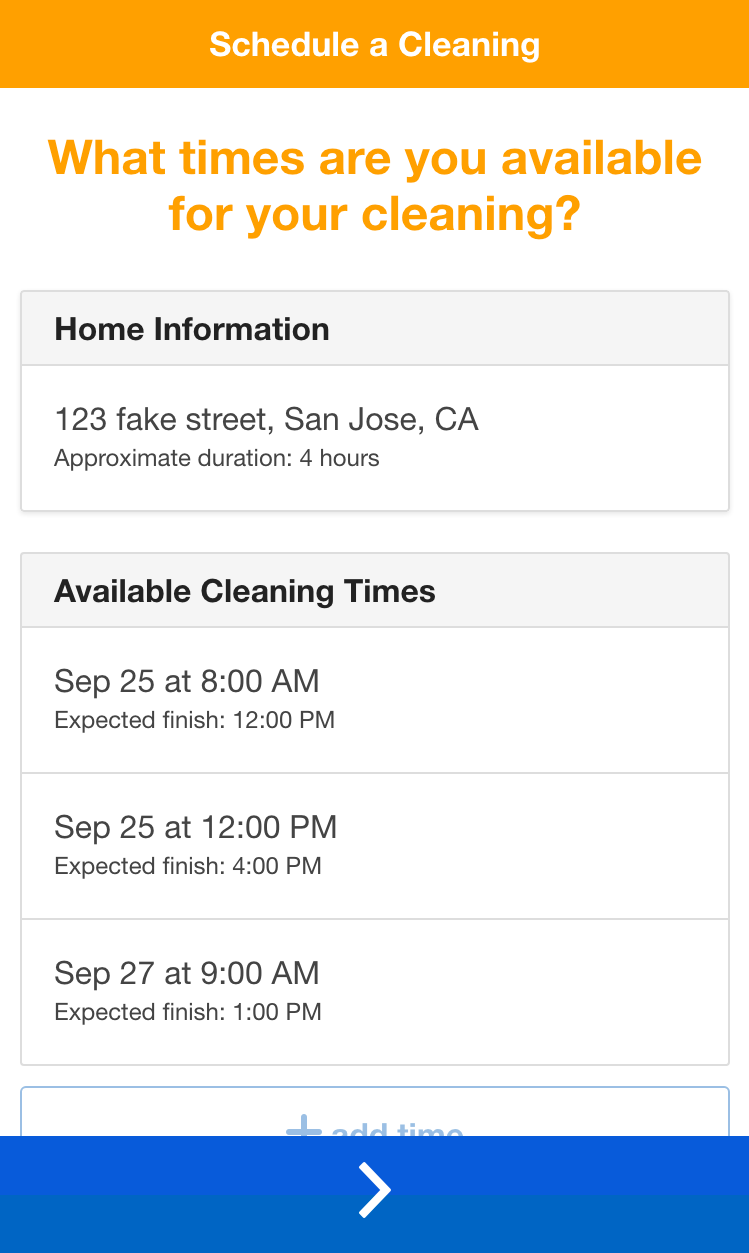
\includegraphics[width=1\columnwidth]{figures/scheduling}
    \caption{In the client's perspective, a lightweight scheduling system can suffice to communicate availability.}~\label{fig:clientSchedule}
\end{figure}
\begin{figure}[t]
\centering
  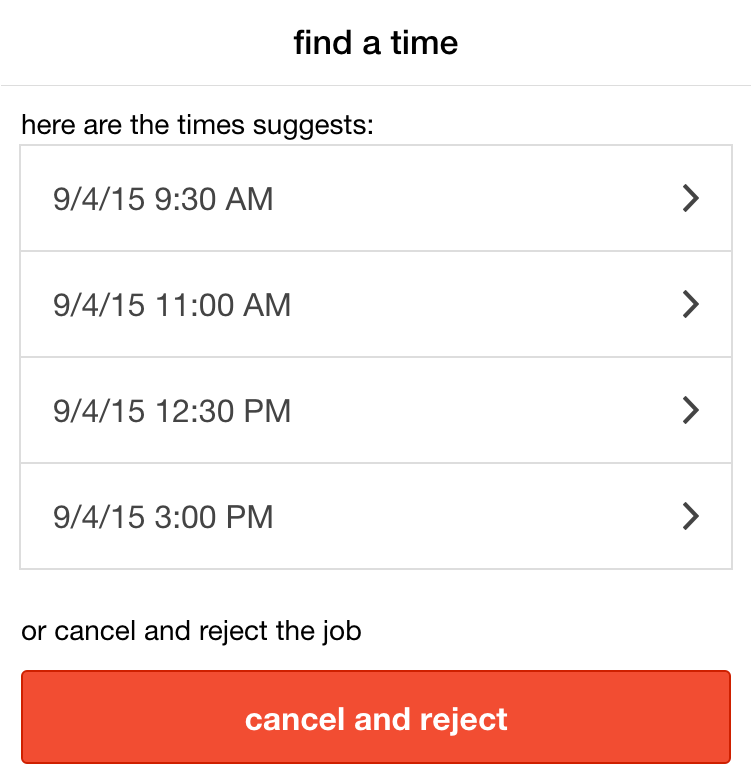
\includegraphics[width=1\columnwidth]{figures/jobtimesoffer}
    \caption{In the worker's perspective, scanning suggested start times can make scheduling easier than entering a series of windows of availability each week or month.}~\label{fig:workerSchedule}
\end{figure}

The task of finding eligible, willing workers can be simplified by considering availability,
narrowing the list of candidate workers to those who are interested in working during a given time frame.
This can, however, be a particularly frustrating challenge for on-demand workers.
One of the most common reasons we heard from gig workers who preferred such work was the flexibility that mode of work offered;
in other words, trying to get workers to commit to windows of availability goes against the nature of that work --- the freedom --- which made it appealing to those we consulted.

This challenge was ameliorated in various ways across field sites; At organization E, workers were assigned each day even if work was solicited days or weeks in advance (unless, of course, a specific worker was requested for repeat work). This process neatly handles the potentially ambiguous question of availability for a number of workers, but it's limiting in two ways:

\begin{enumerate} \itemsep0pt \parskip0pt
  \item organization E's scale is ultimately limited by their ability to process workers on a daily basis (this was particularly salient as a volunteer, processing workers as they arrived to check at 7 A.M.)
  \item Workers who wished to be available for leads had to travel to the organization E offices; sometimes workers would travel north as many as 30 minutes, only to get a job 30 minutes south again.
\end{enumerate}

Instead of setting availability in advance, we suggest optimizing the process of scheduling so that workers and customers spend a minimal amount of time negotiating one another's availability.

This leaves open the question of how that list of workers is determined;
who is the first choice, and who's second if the first worker doesn't claim the job?
Who ends up getting last pick?

We can only offer that this factor is determined in large part by the organization running the system.
A template for a worker-run marketplace should therefore expose these options,
and more importantly surface the debate at the core of these discussions,
while abstracting away the technical details such as implementation.
These cases also illustrate that systems can be designed in ways that meaningfully and fairly reward workers for doing necessary work for the benefit of the community as a whole.
